\documentclass{beamer}
\usepackage{tikz}
\usepackage{lmodern}
\usepackage[absolute,overlay]{textpos}
\usetikzlibrary{shapes,arrows}
\usetikzlibrary{petri}
\usetikzlibrary{automata}

\title{Suppression of Variation in Cell-Size: A Control Theoretic Approach}
\author{Dilawar Singh, Madan Rao}
\begin{document}

\begin{frame}

    \maketitle

    Building over a recent work \cite{paulsson}, we explored the possibility of
    creating networks of small networks which can be utilized for controlling
    cell size. We explored few  topologies in direction of finding a control
    network which can keep the size of the cell fixed and put an upper bound on
    the size of the Endosome. Some progress has been made on building a
    simulator for these topologies in an event-driven simulation environment
    (SystemC library of C++)
    \footnote{https://github.com/dilawar/FeedbackSimulator/}.

\end{frame}

%% Slide 2.
\begin{frame}
    \frametitle{Background}

    \begin{itemize} 
        \item Inside the cell, randomizing and correcting statistical forces
            battle it out and create fluctuations - noise. Many control
            circuits have evolved to eliminate or exploit the noise.  

        \item In this rotation project, we used a recent result \cite{paulsson}
            which establishes limits on 'controllability' in a feedback network
            to build control networks for controlling cell-size.

        \item To explore such network construct, we started building a
            simulation environment using C++ and event-driven simulation library
            \textbf{SystemC}.

    \end{itemize}

    
\end{frame}

\begin{frame}{A Feedback Network Studied in \cite{paulsson}}

    \begin{figure}
        \includegraphics[width=0.5\textwidth]{./fig_mrna_protein.png}
        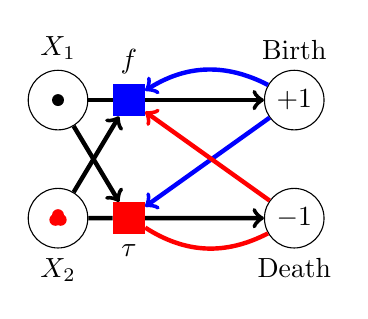
\begin{tikzpicture}[scale=0.3]
        ]
        \node[place,tokens=1,label=above:$X_1$] (X1) at (0,0) {};
        \node[place,colored tokens={red,red,red},label=below:$X_2$] (X2) at (0,-5) {};

        \node[transition,blue,fill,label=above:$f$] (birth) at (3,0) {};
        \node[transition,red,fill,label=below:$\tau$] (death) at (3,-5) {};

        \node[place,label=above:Birth] (Xb) at (10,0) {$+1$};
        \node[place,label=below:Death] (Xd) at (10,-5) {$-1$};


        \draw[ultra thick,->] (X1) to (birth) to (Xb);
        \draw[ultra thick,->] (X1) to  (death);

        \draw[ultra thick,->] (X2) to (death)  to (Xd);
        \draw[ultra thick,->] (X2) to (birth);

        \draw[ultra thick,->,blue] (Xb) to [bend right]  (birth);
        \draw[ultra thick,->,blue] (Xb) to (death);

        \draw[ultra thick,red,->] (Xd) to [bend left] (death) (Xd) to (birth);

    \end{tikzpicture} 

    \caption{\small On left, mRNA/Protein network, from \cite{paulsson}. An
    equivalent description using Petri Nets on the right with $X_1$ as mRNA and
    $X_2$ as its protein. Signalling events are probabilistic.
    } 
\end{figure}

\begin{block}{Birth and Death in Network}
    \begin{eqnarray}
        X_1 \xrightarrow{f'(x_2(-\infty,t))} X_1 + 1 \qquad X_1 \xrightarrow{\tau_{x_1}} X_1 -1 \\
        X_2 \xrightarrow{f(x_1)} X_2 + 1 \qquad X_2 \xrightarrow{\tau_{x_2}} X_2 - 1 
    \end{eqnarray}
\end{block}


\end{frame}

\begin{frame}
    \frametitle{Information theoretic modelling}

    \begin{block}{}
        \emph{How much we can infer about $X_1$ by knowing the time-series of
        $X_2$?}

        The following stochastic equation describes $x_1$.

        \begin{equation}
            \def\mean#1{\left< #1 \right>}
            dx_1 = \frac{f'-x_1}{\tau_1} dt + \sqrt{\frac{2 \mean{x_1}}{\tau_1}}dw
        \end{equation}

    \end{block}


    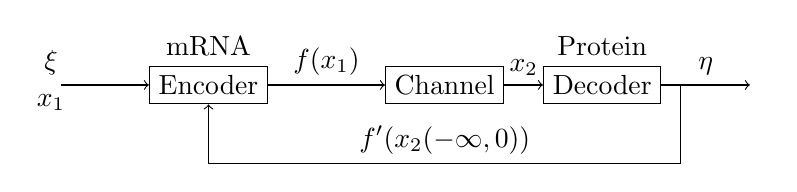
\begin{tikzpicture}[scale=1]
        % This one is information theory approach
        \tikzstyle{block} = [draw,rectangle,];

        \node (input) at (-2,0) {};
        \node (input_midway) at (-1,0) {};
        \node[block,label=above:mRNA ] (encoder) at (0,0) {Encoder};
        \node[block,right of=encoder] (channel)  at (2,0) {Channel};
        \node[block,right of=channel,label=above:Protein] (decoder) at (4,0)  {Decoder};
        \node[right of=decoder,] at (6,0) (output) {};
        \node[right of=decoder,] (output_mid) {};


        \draw[->] (input) node[above] {$\xi$} node[below] {$x_1$} -- (encoder);
        \draw[->] (encoder) -- node[above] {$f(x_1)$} (channel);
        \draw[->] (channel) -- node[above] {$x_2$} (decoder);
        \draw[->] (decoder) --  node[above] {$\eta$} (output);

        \draw[->] (output_mid) -| ++(0,-1) -- ++(-3,0) node[above] {$f'(x_2(-\infty,0))$} -| (encoder);

    \end{tikzpicture}

    \begin{block}{Channel Capacity}
        \def\mean#1{\left< #1 \right>}
        \begin{equation}
            C = \mean{f}\log(1+\frac{\sigma_f^2}{\mean{f}^2})
        \end{equation}
    \end{block}


\end{frame}


\begin{frame}[fragile]
    \frametitle{Information theoretical modelling}
    
    \begin{block}{The bounds}
        \begin{enumerate}
                \small
            \item There is bound on variance in $x_1$ whenever there is a bound
                on error with which $x_1$ can be measured.
            \item To measure $x_1$ with small estimation error, a minimal
                capacity is required for channel $x_1 \rightarrow $.
            \item  To achieve a certain capacity, a minimal variance in the $f$
                is required.
            \item If $f$ depends on $x_1$, then high variance in $x_1$ is needed
                to increase the channel capacity $C$.
        \end{enumerate}

        \emph{Reducing the variance reduces the channel capacity which in turn
        makes is harder to further reduce the variance}.

    \end{block}

    \def\mean#1{\left< #1 \right>}
    \begin{eqnarray}
        \frac{\sigma_{x_1}^2}{\mean{x_1}^2} \geq 
        \frac{1}{\mean{x_1}} \times \frac{2}{1 + \sqrt{1+4N_2/N_1}} \\
        N_1 = \mean{x_1}, N_2 = \mean{f} \tau_1 
    \end{eqnarray}

\end{frame}
 
\begin{frame}
    \frametitle{Network of networks}

    \begin{block}{Cascade of network}

        Put a figure here.

        A linear cascade of networks causes information loss like the game of
        broken-telephone.

        \begin{equation}
            \frac{1}{N_{eff}} = \sum_{j=2}^{n+1} {N_j}^{-1}
        \end{equation}

    \end{block}
\end{frame}

%% Slide where work starts.
\begin{frame}
    \frametitle{Cell-Size control: endocytosis and exocytosis}

    \begin{block}{}
        \begin{itemize}
            \item Size of cell: $X_1$. Size of the endosome: $X_2$.
            \item $U$ is a controller which controls $X1$. 
        \end{itemize}
    \end{block}

    \begin{itemize}
        \item \textbf{Endocytosis} $X_1 \xrightarrow{\tau_{x_1}} X_1 -1$, and $X_2
            \xrightarrow{f(x_1)} X_2 + 1$
        \item \textbf{Exocytosis} $X_1 \xrightarrow{U(x_2(-\infty,t))} X_1 +
            1$, and $X_2 \xrightarrow{\tau_{x_2}} X_2 - 1$.

    \end{itemize}


    \begin{block}{Questions considered}
        \begin{enumerate}
            \item Assume $U$ is most the optimum, what is the variance in
                $X_2$ when $X_1$ is kept at $S_0$?
            \item Assume $U$ is the most optimum, how well network
                controls $X_1$ under random fluctuations (simulation)?
            \item For given benchmarks (fixed $S_0$ and variance in
                $X_2$), can $U$ be designed?
        \end{enumerate}
    \end{block}

\end{frame}

\begin{frame}
    \frametitle{References \& Acknowledgements}

    \begin{thebibliography}{10}
        \bibitem{paulsson}
            Ioannin Lestas., Glenn Vinnicombe, Johan Paulsson
            \newblock {Fundamental limits on the suppression of molecular
            fluctuations}
            \newblock {Nature, Vol 467, Sep 09, 2010}
    \end{thebibliography}

    \begin{block}{}
        
        I'd like to thank Dr. Madan Rao for advice and discussions during the
        rotation; and Amit for walking me through the needed theory. 
        \\
        And various Open Source Softwares especially \LaTeX.

    \end{block}

\end{frame}

\end{document}
